%\documentclass[wcp,gray]{jmlr} % test grayscale version
\documentclass[wcp]{jmlr}

% The following packages will be automatically loaded:
% amsmath, amssymb, natbib, graphicx, url, algorithm2e

%\usepackage{rotating}% for sideways figures and tables
\usepackage{longtable}% for long tables

% The booktabs package is used by this sample document
% (it provides \toprule, \midrule and \bottomrule).
% Remove the next line if you don't require it.
\usepackage{booktabs}
% The siunitx package is used by this sample document
% to align numbers in a column by their decimal point.
% Remove the next line if you don't require it.
%\usepackage[load-configurations=version-1]{siunitx} % newer version
%\usepackage{siunitx}

\usepackage{tikz}

\newcommand{\icon}[1]{\tikz[baseline=-3pt] \node[inner sep=0pt,outer sep=0pt]{\includegraphics[height=1.1em]{images/#1}};}

% The following command is just for this sample document:
\newcommand{\cs}[1]{\texttt{\char`\\#1}}

\jmlrvolume{41}
\jmlryear{2015}
\jmlrworkshop{BIGMINE 2015}

\title[Big Data with ADAMS]{Big Data with ADAMS}

 % Use \Name{Author Name} to specify the name.
 % If the surname contains spaces, enclose the surname
 % in braces, e.g. \Name{John {Smith Jones}} similarly
 % if the name has a "von" part, e.g \Name{Jane {de Winter}}.
 % If the first letter in the forenames is a diacritic
 % enclose the diacritic in braces, e.g. \Name{{\'E}louise Smith}

 % Two authors with the same address
 % \author{\Name{Author Name1} \Email{abc@sample.com}\and
 %  \Name{Author Name2} \Email{xyz@sample.com}\\
 %  \addr Address}

 % Three or more authors with the same address:
 % \author{\Name{Author Name1} \Email{an1@sample.com}\\
 %  \Name{Author Name2} \Email{an2@sample.com}\\
 %  \Name{Author Name3} \Email{an3@sample.com}\\
 %  \Name{Author Name4} \Email{an4@sample.com}\\
 %  \Name{Author Name5} \Email{an5@sample.com}\\
 %  \Name{Author Name6} \Email{an6@sample.com}\\
 %  \Name{Author Name7} \Email{an7@sample.com}\\
 %  \Name{Author Name8} \Email{an8@sample.com}\\
 %  \Name{Author Name9} \Email{an9@sample.com}\\
 %  \Name{Author Name10} \Email{an10@sample.com}\\
 %  \Name{Author Name11} \Email{an11@sample.com}\\
 %  \Name{Author Name12} \Email{an12@sample.com}\\
 %  \Name{Author Name13} \Email{an13@sample.com}\\
 %  \Name{Author Name14} \Email{an14@sample.com}\\
 %  \addr Address}


 % Authors with different addresses:
  \author{\Name{Peter Reutemann} \Email{fracpete@waikato.ac.nz} \\
  \Name{Geoff Holmes} \Email{geoff@waikato.ac.nz}\\
  \addr Department of Computer Science \\
  The University of Waikato \\
  Hamilton, NZ
 }

%\editors{List of editors' names}

\begin{document}

\maketitle

\begin{abstract}
ADAMS is a modular Java framework for developing workflows to be used for
academic research as well as commercial applications. It integrates
data mining applications, like MOA, WEKA, MEKA and R, image and video
processing and feature generation capabilities, spreadsheet and database
access, visualizations, GIS, webservices, fast protoyping of new 
functionality using scripting languages (Jython/Groovy).
\end{abstract}
\begin{keywords}
workflow, big data, data streams, twitter, video, nir
\end{keywords}

\section{Introduction}
The origins of ADAMS lie in academia, with the project getting developed to process analytical data from gas-chromatography mass-spectrometry instruments (\cite{gcms}), handling the many pre-processing steps and various predictions in parallel. However, the ADAMS framework now forms the basis of commercial applications, as it allows for rapid development of data mining applications that integrate into business processes. The framework, written in Java and released under GPLv3, consists of various modules grouped by functionality. It includes MOA, WEKA, MEKA, R, image/video processing and feature generation, spreadsheet and database handling, various visualizations, GIS support through OpenStreetMap, webservices, and scripting (Jython or Groovy) for fast prototyping.

The remainder of the paper is structured as follows: first, a short introduction into the framework is given. Second, a short overview of some of the research areas that it can be used for. Third, a commercial application that is based on the framework.

\section{Framework}
Workflow systems, like RapidMiner, KNIME or Kepler, use a canvas approach for laying out the operators and combining them by connecting them. On the one hand, this is a very intuitive approach, since the user can see how the data flows. On the other hand, this can make modifying the flow a tedious process, as the authors experienced: disconnecting operators, moving them around, inserting other operators, reconnecting operators. Despite birds-eye-view and meta-operators that group several operators together, the canvas approach can quickly become hard to comprehend and doesn't seem to scale well into hundreds or even thousands of operators.

ADAMS forfeits some of the advantages and asthetics of this canvas approach to provide a more compact layout, using a simple tree structure instead for organizing its operators (called actors). The nesting of nodes in the tree resembles the nesting of actors programmatically, based on whether the actor is a primitive one (e.g., filtering a dataset) or one that manages other actors (e.g., grouping actors to be executed sequentially). So-called control actors determine data flow and flow execution: a \icon{Branch} Branch actor forwards the incoming data to all of its sub-actors, i.e., the sub-branches; a \icon{Tee}~Tee actor forkes off data passing through and forwards it to its sub-flow; a \icon{Stop}~Stop actor simply stops the flow execution. The four types of combinations that result from input and output handling, are as follows: \icon{CallableActors}~Standalone, which has no input nor output, e.g., a database connection; \icon{MOAStream}~Source, which only generates output; \icon{MOAClassifierEvaluation}~Transformer, which takes input and generates output; \icon{SequencePlotter}~Sink, which only consumes data. By using data flow control actors, it is possible to get rid of explicit connections between the actors. However, a tree structure only handles 1-to-n connections. In order to simulate n-to-m semantics, several techniques are implemented: use of containers to combine multiple outputs; support for variables, to be attached to parameters of actors or simply used for calculations; internal key-value storage for storing, retrieving and updating data in multiple locations; callable actors can be invoked from anywhere in the flow. Interoperability of actors is statically checked by comparing the types of data that a preceding actor can output and what types the following actor can handle. This type information in combination with the context induced by the tree structure, makes it possible to limit the actors that can be placed within this context. Furthermore, context-aware rules can be specified for common sequences of actors (load dataset $\rightarrow$ set class attribute $\rightarrow$ cross-validate dataset $\rightarrow$ output results) aiding the user in creating flows more rapidly.

\begin{figure}[htb]
  \begin{minipage}[b]{0.5\linewidth}
  \centering
  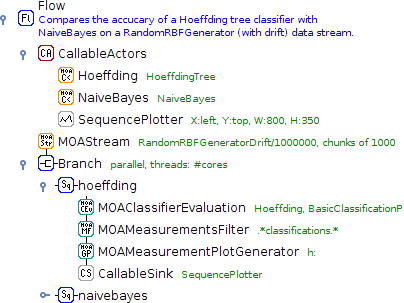
\includegraphics[width=7.0cm]{images/example_flow_clipped.png}
  \caption{Comparing two MOA classifiers.}
  \label{example_flow}
  \end{minipage}%
  \begin{minipage}[b]{0.5\linewidth}
  \centering
  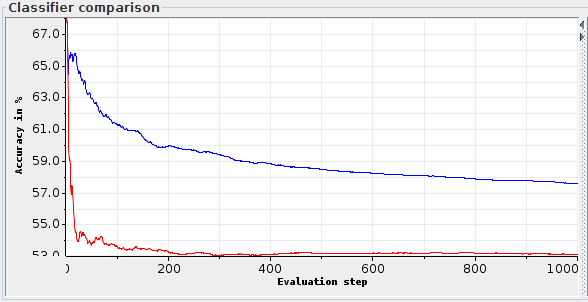
\includegraphics[width=8.0cm]{images/example_output_clipped.png}
  \caption{Comparison output.}
  \label{example_output}
  \end{minipage}
\end{figure}

\section{Research}
- moa: stream analysis, filtering, visualization
- moa: classification, regression, clustering
- twitter: collecting of tweets using public API, replay of tweets for testing/comparing different algorithms (same stream!)
- video analysis (webcam/movie): object tracking for rat monitoring (upcoming with Biology department)

\section{Industry}
spectral analysis
\begin{itemize}
 \item meta-flows, flow generators
 \item raw xrf 10k att, mir 2k, nir 1.5k
 \item nir model 150k instances (soil)
 \item soil season 2-3k/d
 \item num models 250 models (soil/plant)
 \item savings: nir 17million euro/a, soil season 30million euro/a (every 4 years)
 \item since 2006 in place
\end{itemize}
\cite{mlmatters}

\acks{The authors would like to thank the organizers, especially Albert Bifet, for inviting us to present our work.}

\bibliography{bigmine15-adams-paper}

\end{document}
